\documentclass[12pt]{extreport} % Schriftgröße: 8pt, 9pt, 10pt, 11pt, 12pt, 14pt, 17pt oder 20pt

%% Packages
\usepackage{scrextend}
\usepackage{amssymb}
\usepackage{amsthm}
\usepackage{booktabs}
\usepackage{caption}
\usepackage{subcaption}
\usepackage{chngcntr}
\usepackage{cmap}
\usepackage{color}
\usepackage{csquotes}
\usepackage{enumitem}
\usepackage{float}
\usepackage{graphicx}
\usepackage{hyperref}
\usepackage{ulem}
\usepackage{lmodern}
\usepackage{makeidx}
\usepackage{amsmath}
\usepackage{mathtools}
\usepackage{xpatch}
\usepackage{pgfplots}
\pgfplotsset{compat=1.7}
\usetikzlibrary{calc}	
\usetikzlibrary{matrix}	

% Language Setup (English)
\usepackage[utf8]{inputenc} 
\usepackage[T1]{fontenc} 
\usepackage[english]{babel}

% Options
\makeatletter%%  
  % Linkfarbe, {0,0.35,0.35} für Türkis, {0,0,0} für Schwarz, {1,0,0} für Rot, {0,0,0.85} für Blau
  \definecolor{linkcolor}{rgb}{0,0.35,0.35}
  % Zeilenabstand für bessere Leserlichkeit
  \def\mystretch{1.2} 
  % Publisher definieren
  \newcommand\publishers[1]{\newcommand\@publishers{#1}} 
  % Enumerate im 1. Level: \alph für a), b), ...
  \renewcommand{\labelenumi}{\alph{enumi})} 
  % Enumerate im 2. Level: \roman für (i), (ii), ...
  \renewcommand{\labelenumii}{(\roman{enumii})}
  % Zeileneinrückung am Anfang des Absatzes
  \setlength{\parindent}{0pt} 
  % Für das Proof-Environment: 'Beweis:' anstatt 'Beweis.'
  \xpatchcmd{\proof}{\@addpunct{.}}{\@addpunct{:}}{}{} 
  % Nummerierung der Bilder, z.B.: Abbildung 4.1
  \@ifundefined{thechapter}{}{\def\thefigure{\thechapter.\arabic{figure}}} 
  % Chapter-Nummerierung beginnen bei (0):
  \setcounter{chapter}{0}
  % Chapter-Nummerierung
  \renewcommand\thechapter{\Roman{chapter}}
\makeatother%

% Meta Setup 
\title{Asset Pricing}
\author{Prof. Marliese Uhrig-Homburg}
\date{Sommersemester 2017}
\publishers{Karlsruher Institut für Technologie}

%% Math. Definitiones
\newcommand{\C}{\mathbb{C}}
\newcommand{\N}{\mathbb{N}}
\newcommand{\Q}{\mathbb{Q}}
\newcommand{\R}{\mathbb{R}}
\newcommand{\Z}{\mathbb{Z}}
\newcommand{\DO}[1]{\mathcal{D}\left( {#1} \right)}
\newcommand{\RO}[1]{\mathcal{R}\left( {#1} \right)}

\newtheoremstyle{named}{}{}{\normalfont}{}{\bfseries}{:}{0.25em}{#2 \thmnote{#3}}
\newtheoremstyle{nnamed}{}{}{\normalfont}{}{\bfseries}{:}{0.25em}{\thmnote{#3}}
\newtheoremstyle{itshape}{}{}{\itshape}{}{\bfseries}{:}{ }{}
\newtheoremstyle{normal}{}{}{\normalfont}{}{\bfseries}{:}{ }{}
\renewcommand*{\qed}{\hfill\ensuremath{\square}}

\theoremstyle{named}
\newtheorem{unnamedtheorem}{Theorem} \counterwithin{unnamedtheorem}{chapter}
\theoremstyle{nnamed}
\newtheorem*{unnamedtheorem*}{Theorem} 

\theoremstyle{itshape}
\newtheorem{definition}[unnamedtheorem]{Definition}

\theoremstyle{normal}
\newtheorem*{recall}{Recall}
\newtheorem*{example}{Example}
\newtheorem*{remark}{Remark}
\newtheorem*{satz}{Satz}
\newtheorem*{bemerkung}{Bemerkung}

%% Template
\makeatletter%
\DeclareUnicodeCharacter{00A0}{ } \pgfplotsset{compat=1.7} \hypersetup{colorlinks,breaklinks, urlcolor=linkcolor, linkcolor=linkcolor, pdftitle=\@title, pdfauthor=\@author, pdfsubject=\@title, pdfcreator=\@publishers}\DeclareOption*{\PassOptionsToClass{\CurrentOption}{report}} \ProcessOptions \def\baselinestretch{\mystretch} \setlength{\oddsidemargin}{0.125in} \setlength{\evensidemargin}{0.125in} \setlength{\topmargin}{0.5in} \setlength{\textwidth}{6.25in} \setlength{\textheight}{8in} \addtolength{\topmargin}{-\headheight} \addtolength{\topmargin}{-\headsep} \def\pulldownheader{ \addtolength{\topmargin}{\headheight} \addtolength{\topmargin}{\headsep} \addtolength{\textheight}{-\headheight} \addtolength{\textheight}{-\headsep} } \def\pullupfooter{ \addtolength{\textheight}{-\footskip} } \def\ps@headings{\let\@mkboth\markboth \def\@oddfoot{} \def\@evenfoot{} \def\@oddhead{\hbox {}\sl \rightmark \hfil \rm\thepage} \def\chaptermark##1{\markright {\uppercase{\ifnum \c@secnumdepth >\m@ne \@chapapp\ \thechapter. \ \fi ##1}}} \pulldownheader } \def\ps@myheadings{\let\@mkboth\@gobbletwo \def\@oddfoot{} \def\@evenfoot{} \def\sectionmark##1{} \def\subsectionmark##1{}  \def\@evenhead{\rm \thepage\hfil\sl\leftmark\hbox {}} \def\@oddhead{\hbox{}\sl\rightmark \hfil \rm\thepage} \pulldownheader }	\def\chapter{\cleardoublepage  \thispagestyle{plain} \global\@topnum\z@ \@afterindentfalse \secdef\@chapter\@schapter} \def\@makeschapterhead#1{ {\parindent \z@ \raggedright \normalfont \interlinepenalty\@M \Huge \bfseries  #1\par\nobreak \vskip 40\p@ }} \newcommand{\indexsection}{chapter} \patchcmd{\@makechapterhead}{\vspace*{50\p@}}{}{}{}\def\Xint#1{\mathchoice
    {\XXint\displaystyle\textstyle{#1}} {\XXint\textstyle\scriptstyle{#1}} {\XXint\scriptstyle\scriptscriptstyle{#1}} {\XXint\scriptscriptstyle\scriptscriptstyle{#1}} \!\int} \def\XXint#1#2#3{{\setbox0=\hbox{$#1{#2#3}{\int}$} \vcenter{\hbox{$#2#3$}}\kern-.5\wd0}} \def\dashint{\Xint-} \def\Yint#1{\mathchoice {\YYint\displaystyle\textstyle{#1}} {\YYYint\textstyle\scriptscriptstyle{#1}} {}{} \!\int} \def\YYint#1#2#3{{\setbox0=\hbox{$#1{#2#3}{\int}$} \lower1ex\hbox{$#2#3$}\kern-.46\wd0}} \def\YYYint#1#2#3{{\setbox0=\hbox{$#1{#2#3}{\int}$}  \lower0.35ex\hbox{$#2#3$}\kern-.48\wd0}} \def\lowdashint{\Yint-} \def\Zint#1{\mathchoice {\ZZint\displaystyle\textstyle{#1}}{\ZZZint\textstyle\scriptscriptstyle{#1}} {}{} \!\int} \def\ZZint#1#2#3{{\setbox0=\hbox{$#1{#2#3}{\int}$}\raise1.15ex\hbox{$#2#3$}\kern-.57\wd0}} \def\ZZZint#1#2#3{{\setbox0=\hbox{$#1{#2#3}{\int}$} \raise0.85ex\hbox{$#2#3$}\kern-.53\wd0}} \def\highdashint{\Zint-} \DeclareRobustCommand*{\onlyattoc}[1]{} \newcommand*{\activateonlyattoc}{ \DeclareRobustCommand*{\onlyattoc}[1]{##1} } \AtBeginDocument{\addtocontents{toc} {\protect\activateonlyattoc}} \newcommand{\RightArrow}{\xRightarrow[]{ ~ ~ }} \newcommand{\LeftArrow}{\xLeftarrow[]{ ~ ~ }} \newcommand{\rightArrow}{\xrightarrow[]{ ~ ~ }} \newcommand{\leftArrow}{\xleftarrow[]{ ~ ~ }}
	% Titlepage
	\def\maketitle{ \begin{titlepage} 
			~\vspace{3cm} 
		\begin{center} {\Huge \@title} \end{center} 
	 		\vspace*{1cm} 
	 	\begin{center} {\large \@author} \end{center} 
	 	\vspace*{-0.5cm}
	 	\begin{center} \@date \end{center} 
	 		\vspace*{7cm} 
	 	\begin{center} \@publishers \end{center} 
	 		\vfill 
	\end{titlepage} }
\makeatother%

% Create Index
\makeindex 

\begin{document}

\thispagestyle{empty}

% Lecture Notes - Start 			
\pagenumbering{arabic}

\subsection*{Aufgabe S.1} ~\\

\begin{figure}[h!]
  \centering
  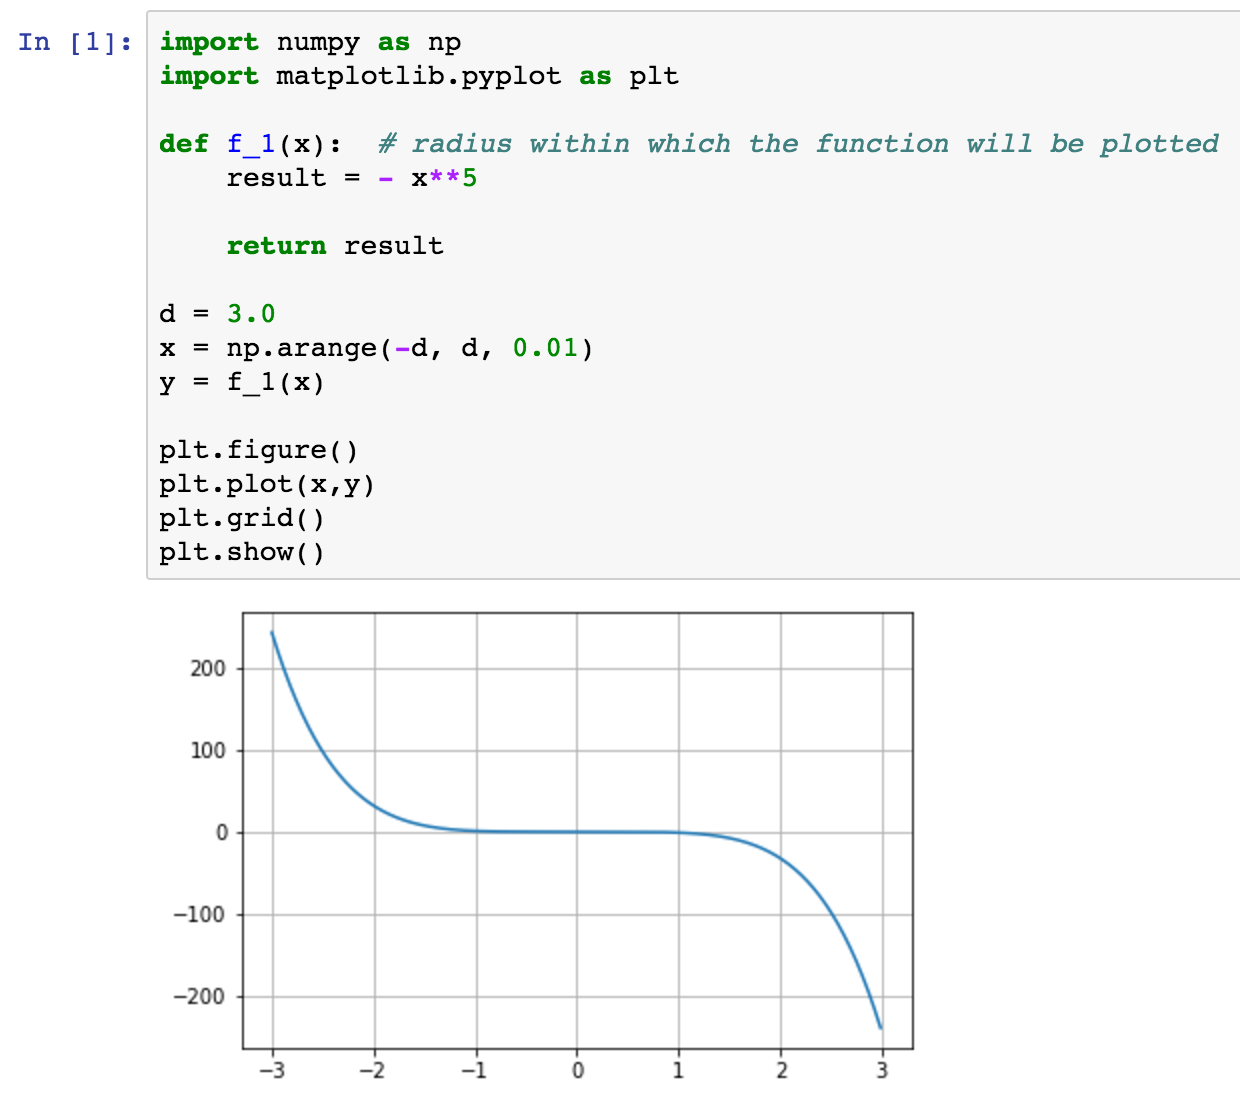
\includegraphics[scale=0.325]{img/sui-i}
  \label{fig:sub1}
\end{figure} ~\\

\begin{figure}[h!]
  \centering
  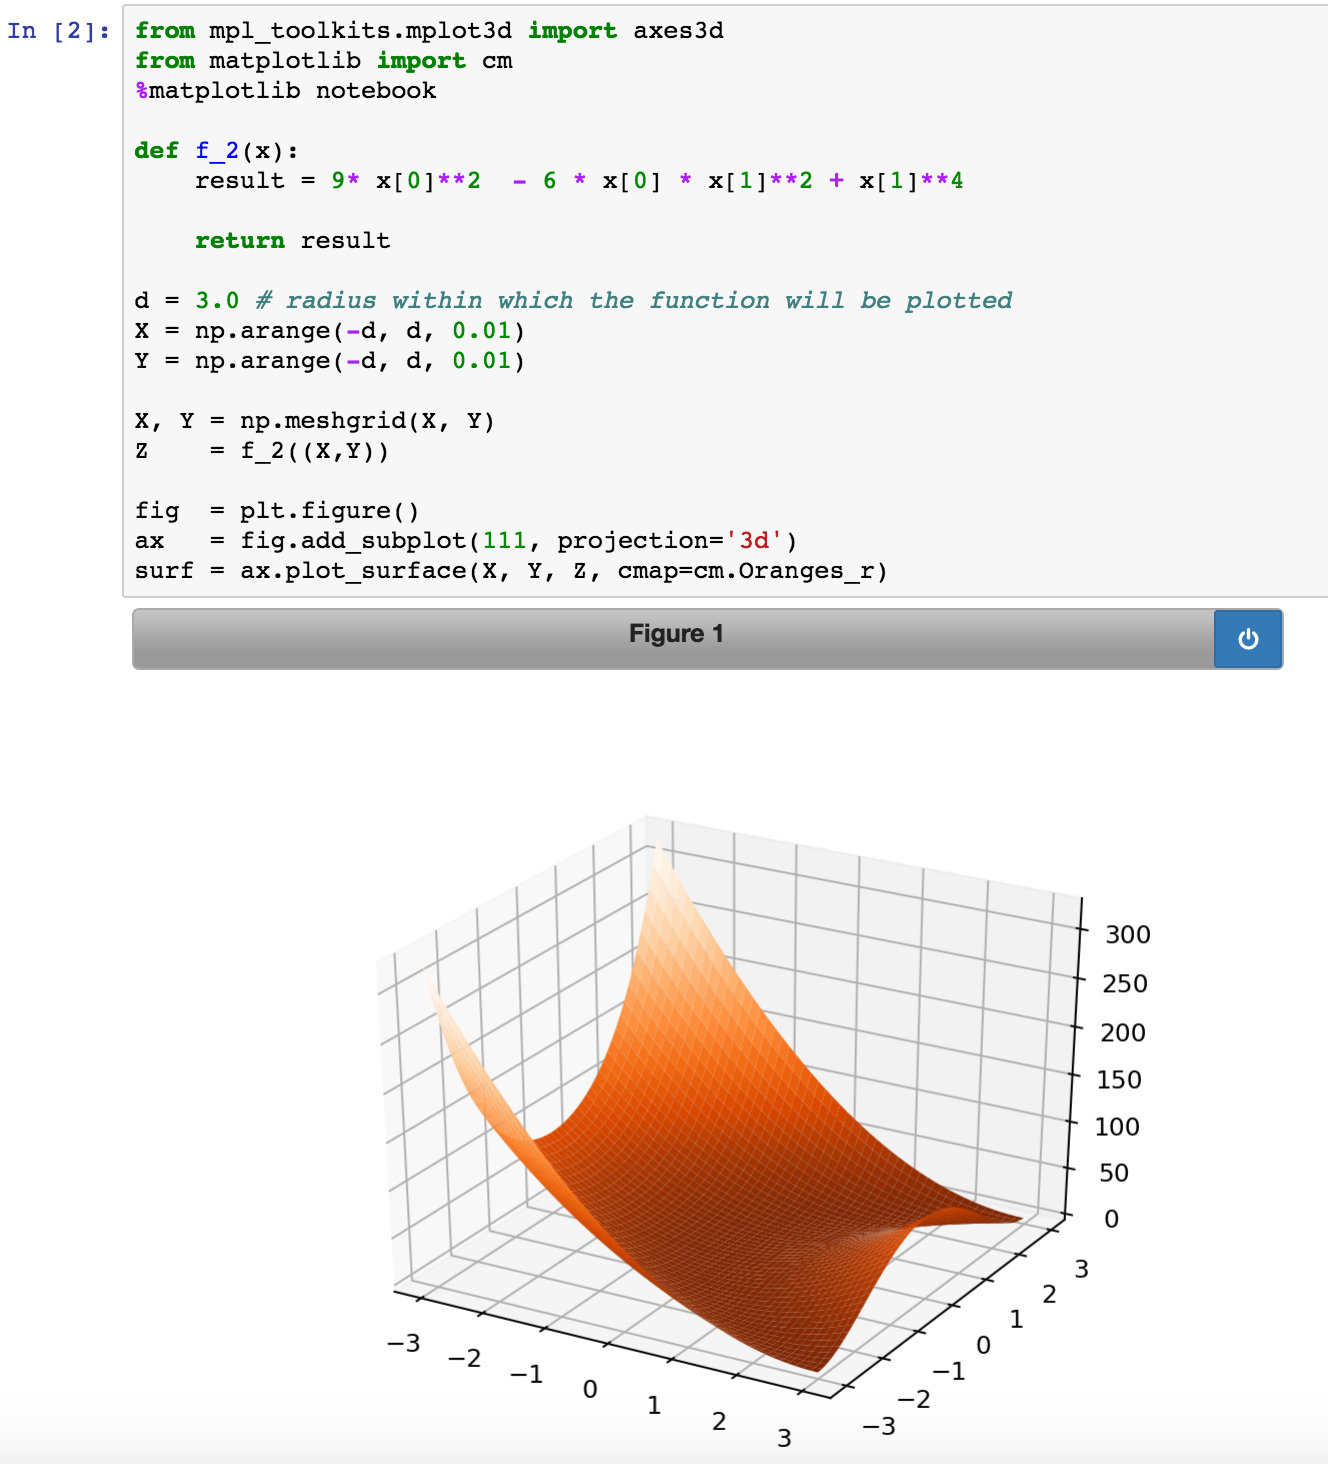
\includegraphics[scale=0.35]{img/sui-ii}
  \label{fig:sub2}
\end{figure}

\newpage

\subsubsection{Aufgabe S.2} ~\\
Gegeben sei das Optimierungsproblem
$$ P: \quad \min f(x), \text{ s.t. } x \in M $$
mit
\begin{enumerate}
	\item $f(x) = - x^5$, $M =(- \infty, 1)$.
	\item $f(x) = 9 x_1^2 - 6 x_1 x_2^2 + x_2^4$, $M = \R^2$
	\item $f(x) = \frac{x^T A x}{\| x - b\|_2 + 1}$, mit $A \in \R^{n \times n}$ positiv definit, $b \in \R^n$ und $M = \R^n$.
\end{enumerate}
	Begründen Sie jeweils: ist $f$ koerziv auf $M$? Ist $P$ lösbar? ~\\
	\textbf{Hinweis}: Nutzen Sie für Aufgabenteil c) die Äquivalenz der Normen im $\R^n$ ~\bigskip

\begin{proof} Nach Vorlesung (Definition 1.2.37) gilt: ~\\ ~\medskip
	\textit{Gegeben seien eine (nicht notwendigerweise abgeschlossene) Menge $M \subseteq \R^n$ und eine Funktion $f \colon M \rightarrow \R$. Falls für alle Folgen $(x^\nu) \subseteq M$ mit $\lim_{\nu} \| x^\nu \| \rightarrow \infty$ und alle konvergenten Folgen $(x^\nu) \subseteq M$ mit $\lim_{\nu} x^\nu \notin M$ die Bedingung}
	$$ \lim_{\nu} f(x^\nu) = + \infty $$
	\textit{gilt, dann heißt $f$ koerziv auf $M$.} ~\\
	
	\begin{enumerate} % todo Lösbar
		\item $f(x) = - x^5$, $M =(- \infty, 1)$: ~\medskip
		
			Beachte $M \subseteq \R$. Es gilt $\overline{M} = (-\infty, 1]$, d.h. $\partial M = \{ 1 \}$. Für die Koerzivität sind demnach alle Folgen $\left( x^\nu \right) \subseteq M$ zu betrachten für die entweder
			$$ x^\nu \longrightarrow \infty \quad \text{oder} \quad x^\nu \longrightarrow 1 $$
			gilt. Sei nun $(x^\nu)$ eine Folge für die gilt $x^\nu \rightarrow 1$. Für alle $\epsilon > 0$ existiert demnach ein $m$, sodass:
			$$ \| x^{\nu_m} - 1 \| < \epsilon, \quad \forall \nu_m > m. $$
			Daraus ergibt sich:
			\begin{align*}
				 \lim_\nu f(x^\nu) = \lim_\nu \left( - \left(x^\nu \right)^5 \right) & = -  \lim_\nu \left( \left(x^\nu - 1 + 1 \right)^5 \right) \\
				 	& \leq - \lim_\nu  \left( - \left( \| x^\nu -1 \| + 1 \right)^5 \right) \\
				 	& < \lim_\nu  \left( \epsilon + 1 \right)^5.  
			\end{align*}
			Da diese Ungleichung im Grenzwert für alle $\epsilon > 0$ gilt, ist $f$ nicht koerziv. ~\\ 
		\item  $f(x) = 9 x_1^2 - 6 x_1 x_2^2 + x_2^4$, $M = \R^2$: ~\medskip
		
			Es gilt
			$$ f(x) = 9 x_1^2 - 6 x_1 x_2^2 + x_2^4 = (3 x_1 - x_2^2)^2. $$
			Demnach ist für jede Folge für die gilt $\sqrt{3 x^\nu_1} = x^\nu_2$ für alle $\nu \in \N$:
			$$ f(x^\nu) = 0. $$
			Da wir eine Menge von Folgen gefunden haben für die $\| x^\nu \| \rightarrow \infty$ gilt, allerdings gleichzeitig $\lim_{\nu} f(x^\nu) = f(x^{\tilde{\nu}}) = 0$, ist die Funktion nicht koerziv. ~\\ 
		\item $f(x) = \frac{x^T A x}{\| x - b\|_2 + 1}$, mit $A \in \R^{n \times n}$ positiv definit, $b \in \R^n$ und $M = \R^n$: ~\medskip
		
			Da $\R^{n \times n}$ unbeschränkt ist, betrachten wir lediglich eine beliebige divergente Folge $(x^\nu)$. Aufgrund der positiven Definitheit von $A$ ist $ x^T A x > 0$ und damit ist
			$$ f(x) = \frac{x^T A x}{\| x - b\|_2 + 1} > 0.$$ 
			In der Übung wurde die Norm
			$$ \| x \|_{\tilde{A}} = \sqrt{\langle x, x \rangle_{\tilde{A}}} = \sqrt{x^T \tilde{A} x} $$
			eingeführte, mit einer positiv definite, symmetrische Matrix $\tilde{A}$. Wir können o.B.d.A. annehmen, dass die positiv definite Matrix $A$ aus der Aufgabe auch symmetrisch ist, denn es gilt
			$$ x^T A x = x^T \left( \frac{A^T + A}{2} \right) x, $$
			und $\frac{A^T + A}{2}$ ist symmetrisch (ansonsten ersetze $A$ durch $\frac{A^T + A}{2}$). Damit folgt:
			$$ \left| f(x^\nu) \right| =  \left| \frac{\left(x^\nu \right)^T A x^\nu }{\| x^\nu - b\|_2 + 1} \right| = \frac{\left\| x^\nu \right\|_{A}^2}{\| x^\nu - b\|_2 + 1}. $$
			Aufgrund der Divergenz der Folge $(x^\nu)$ gilt für $\nu$ groß genug unter Verwendung der Dreiecksungleichung die Abschätzung
			\begin{align*}
				 \left| f(x^\nu) \right| =  \frac{\left\| x^\nu \right\|_{A}^2}{\| x^\nu - b\|_2 + 1} & \geq \frac{\left\| x^\nu \right\|_{A}^2}{2 \| x^\nu - b\|_2 } \\
				 	& \geq \frac{\left\| x^\nu \right\|_{A}^2}{2 \left( \| x^\nu \|_2 + \| b\|_2 \right)}   \\
				 	& \geq \frac{\left\| x^\nu \right\|_{A}^2}{2 \left( \| x^\nu \|_2 + \| x^\nu \|_2 \right)}  
			\end{align*}
			Durch die Äquivalenz der Normen im $\R^n$ existiert nun eine Konstante $c$ so, dass
			$$ 		\left| f(x^\nu) \right|  \geq \frac{c}{2} \cdot \frac{\left\| x^\nu \right\|_{A}^2}{2 \left( \| x^\nu \|_A + \| x^\nu \|_A \right)} = \frac{c}{4} \cdot \frac{\left\| x^\nu \right\|_{A}^2}{ \| x^\nu \|_A} = \frac{c}{4} \cdot \| x^\nu \|_A \rightarrow \infty, $$
			wobei wir im letzten Schritt wieder die Äquivalenz der Normen verwendet haben, da somit $x^\nu$ in allen Normen divergiert. Das heißt, für alle divergenten Folgen $(x^\nu)$, ist $f(x^\nu) > 0$ und
			$$ \left| f(x^\nu) \right| \rightarrow \infty, $$
			d.h. $f$ ist koerziv.
	\end{enumerate}
\end{proof}

\newpage

\subsubsection{Aufgabe S.3} ~\\
Gegeben sei das unrestringierte Optimierungsproblem
$$ P : \quad \min_{x \in \R^2} \exp \left(- \min{- x_1 - 3, -\left|x_2 - 4\right|, x_1 + x_2 - 20} \right).$$
\begin{enumerate}
	\item Geben Sie die verallgemeinerte Epigraph-Umformulierung $P_{epi}$ von $P$ an (siehe Übung 1.3.9. im Skript). Begründen Sie, welche Funktionen $f$, $g$, $F$ und $G$ Sie für die Umformulierung verwenden.
		\begin{proof}
			Da es sich um ein unrestringiertes Problem handelt, ist $X = \R^2$, $G \equiv 0, g \equiv 0$. Definiere
			\begin{align*}
				& F: \R \rightarrow \R, x \mapsto e^{-x}, \\
				&f: R^2 \rightarrow R, x \mapsto \min\{- x_1 - 3, -\left|x_2 - 4\right|, x_1 + x_2 - 20\}. \\
			\end{align*}
			Damit ist das unrestringierte Optimierungsproblem äquivalent zu
			$$ P : \quad \min_{x \in \R^2} F(f(x)) \text{ s.t. } G(g(x)) \leq 0, x \in X $$
			Nach Übung 1.3.9 (Verallgemeinerte Epigraph-Umformulierung) ist somit folgende Epigraph-Umformulierung äquivalent zu $P$:
			$$ P_{epi}: \min_{(x, \alpha, \beta) \in \R^2 \times R \times \R} F(\alpha) \text{ s.t. } G(\beta) \leq 0, f(x) \leq \alpha, g(x) \leq \beta, x \in X $$
			$$ \iff \min_{(x, \alpha) \in \R^2 \times R} e^{-\alpha} \text{ s.t. } \min\{- x_1 - 3, -\left|x_2 - 4\right|, x_1 + x_2 - 20\} \leq \alpha, x \in X $$
		\end{proof}
	\item Formulieren Sie, aufbauend auf Aufgabenteil a), ein lineares Optimierungsproblem $P_{lin}$, welches die selben Optimalpunkte wie $P_{epi}$ besitzt.
		\begin{proof}
			Sei
			\begin{align*}
				& \tilde{F}: \R \rightarrow \R, x \mapsto e^{x}, \\
				&\tilde{f}: R^2 \rightarrow R, x \mapsto -\min\{- x_1 - 3, -\left|x_2 - 4\right|, x_1 + x_2 - 20\}. \\
			\end{align*}
			Dann ist $F(f(x)) = \tilde{F}(\tilde{f}(x))$ für alle $x \in X$. D.h. $\tilde{F}$, $\tilde{f}$ beschreiben das gleiche Optimierungsproblem und es gilt
			$$ \tilde{f}(x) = -\min\{- x_1 - 3, -\left|x_2 - 4\right|, x_1 + x_2 - 20\} =  \max\{ x_1 + 3, \left|x_2 - 4\right|, -(x_1 + x_2) + 20\}.  $$
			Die Bedingung $\tilde{f}(x) \leq \alpha$ der Epigraph-Formulierung bedeutet für $\tilde{f}$, dass jede Komponente des Maximums kleiner gleich $\alpha$ sein muss, d.h.
			$$  \tilde{P}_{epi}: \min_{(x, \alpha) \in \R^2 \times R} e^{\alpha} \text{ s.t. } x \in X, \begin{cases} x_1 + 3 \leq \alpha \\
			 x_2 - 4 \leq \alpha, ~ - x_2 + 4 \geq - \alpha \\ -(x_1 + x_2) + 20 \leq \alpha \end{cases} $$
			 Da die Exponentialfunktion zudem streng monoton ist, ist jedes Minimum der Identität auf dieser Menge gleich dem Minimum der Exponentialfunktion, d.h. ein lineares Optimierungsproblem $P_{lin}$, welches die selben Optimalpunkte wie $P_{epi}$ besitzt, lautet
			$$  \tilde{P}_{epi}: \min_{(x, \alpha) \in \R^2 \times R} \alpha \text{ s.t. } x \in X, \begin{cases} x_1 + 3 \leq \alpha \\
			 x_2 - 4 \leq \alpha, ~ - x_2 + 4 \geq - \alpha \\ -(x_1 + x_2) + 20 \leq \alpha \end{cases} $$			 
		\end{proof}
	\item Zeigen Sie, mit Hilfe des verschärften Satz von Weierstraß, dass das Problem $P_lin$ lösbar ist.
	\item Modellieren Sie das Problem in Matlab/ Jupyter Notebook und geben Sie den globalen Minimalpunkt von $P_{lin}$ aus.
	\item Bestimmen Sie einen globalen Optimalpunkt und den Optimalwert von P.
\end{enumerate}

\end{document}